% ------------------------------------------------------------------------------
% ANEXO
% Existe adicionalmente el entorno \begin{appendixd} que permite insertar
% \chapter y el entorno \begin{appendixdtitle}[style1] (4 estilos diferentes),
% el cual acepta \chapter y escribe el título de anexos encima
% ------------------------------------------------------------------------------
\begin{appendixs}
	
	\section{Additional DDPO samples}\label{appendix:additional-samples}

    \textbf{Additional samples.} A hundred additional comparable samples from the pretrained and DDPO finetuned models are provided.

        % 100 samples from the pretrained model
        \begin{figure}[ht]
            \centering
            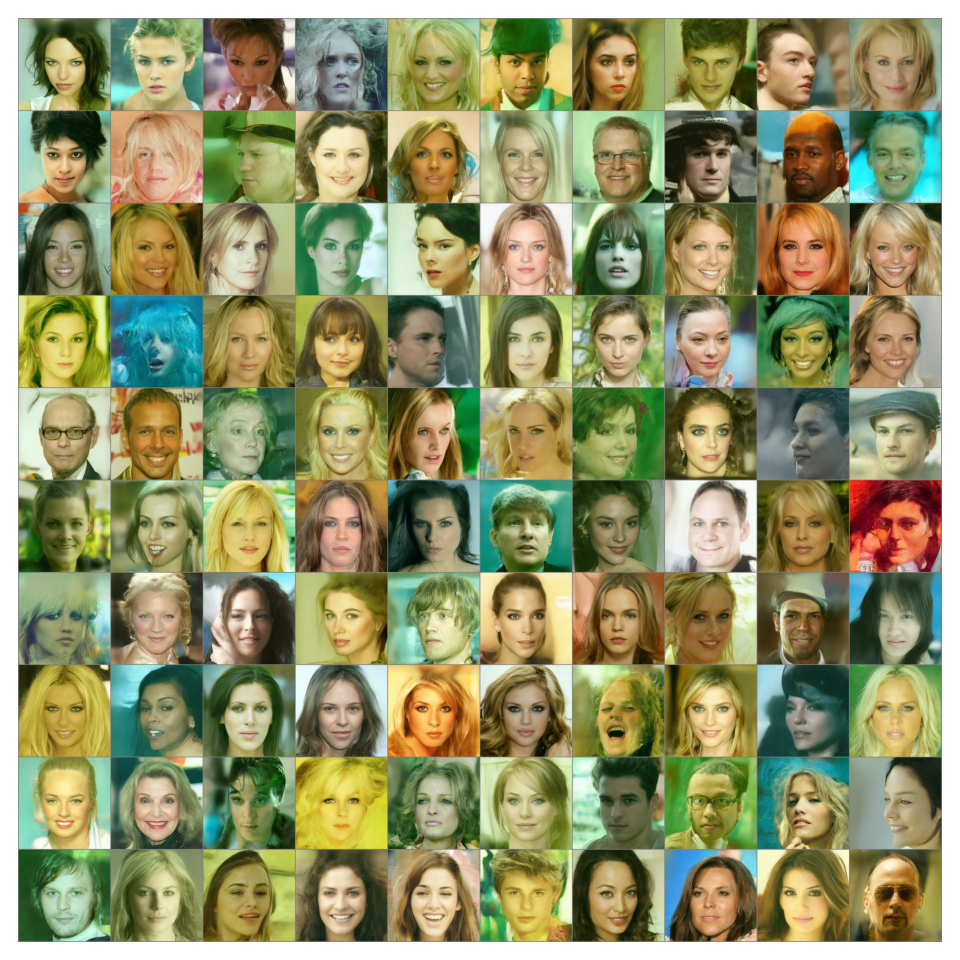
\includegraphics[scale=0.75]{img/results/ddpm-samples.png}
            \vspace{-4pt}  % reduce space between caption and figure
            \captionsetup{width=\textwidth} % set the width of the caption
            \caption{Celeba-HQ 256x256 generated samples from the pretrained model google/ddpm-celebahq-256.}
            \label{fig:ddpm-samples}
        \end{figure}

        % 100 samples from the finetuned model with ddpo and compressibility
        \begin{figure}
            \centering
            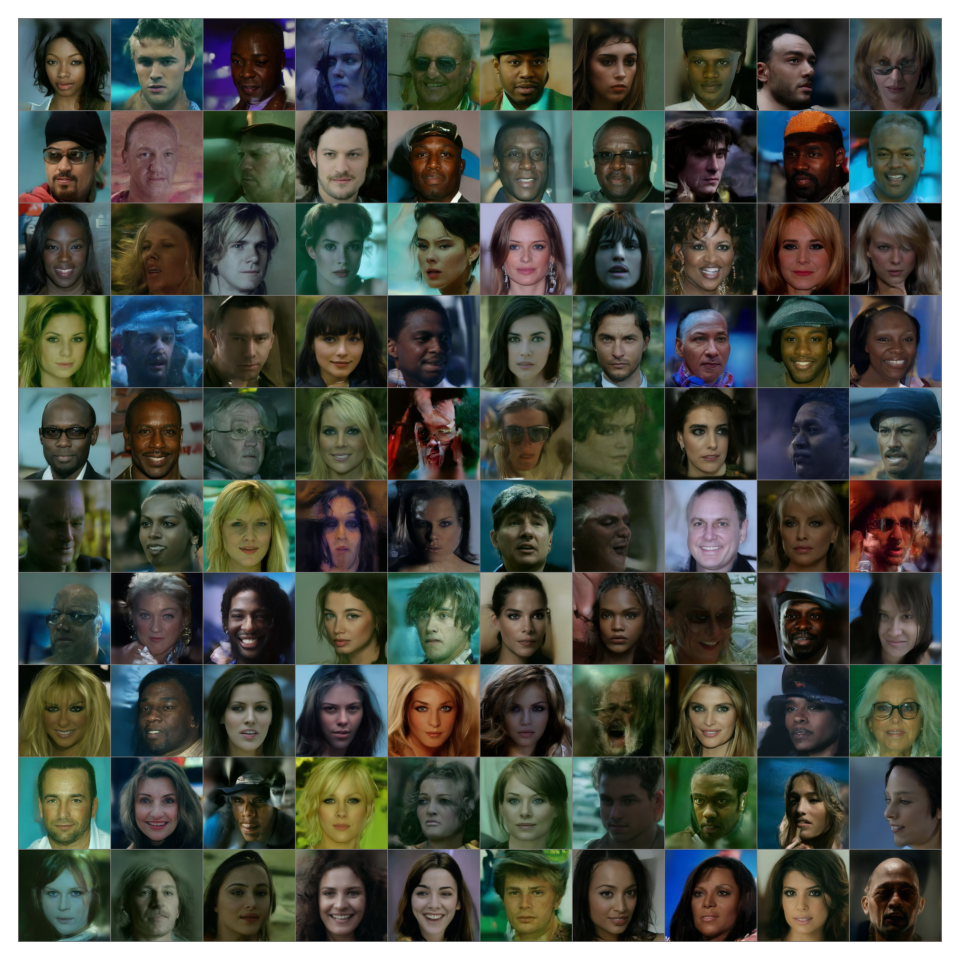
\includegraphics[scale=0.75]{img/results/ddpo-compressibility-samples.png}
            \vspace{-4pt}  % reduce space between caption and figure
            \captionsetup{width=\textwidth} % set the width of the caption
            \caption{Celeba-HQ 256x256 generated samples from the DDPO finetuned model optimized by JPEG compressibility.}
            \label{fig:ddpo-compressibility-samples}
        \end{figure}

        % 100 samples from the finetuned model with ddpo and incompressibility
        \begin{figure}
            \centering
            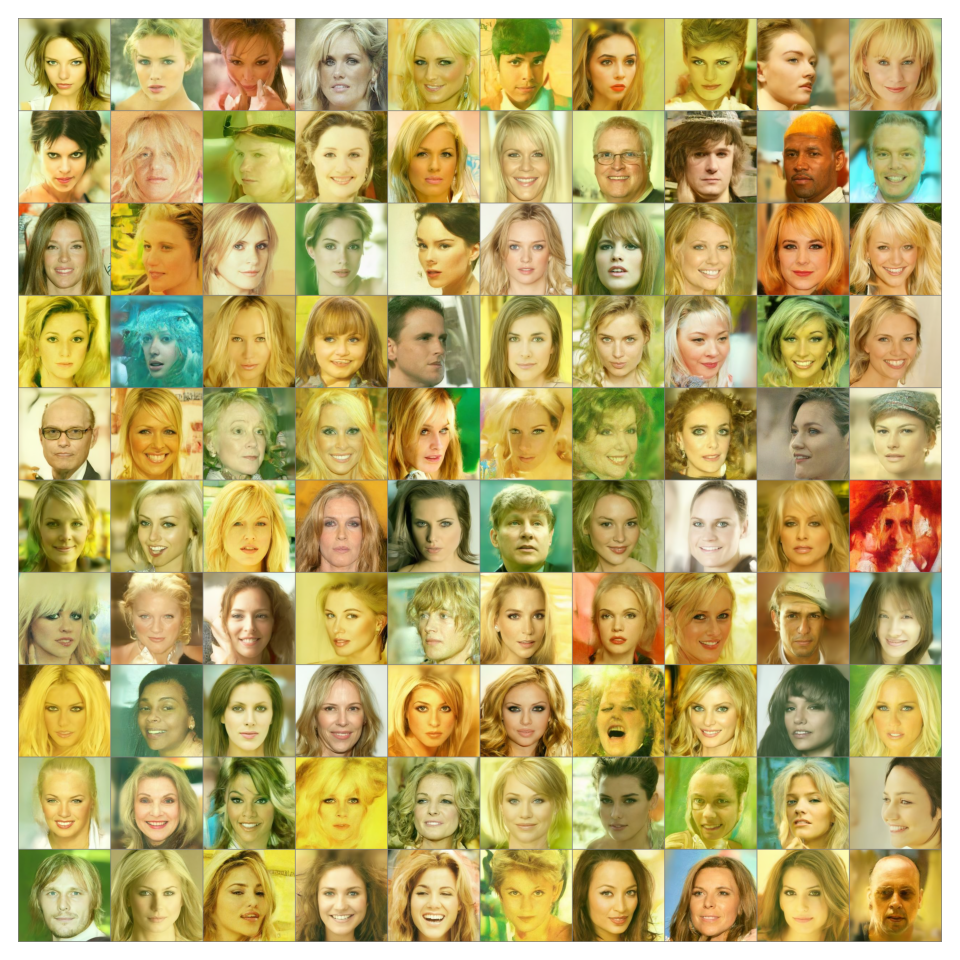
\includegraphics[scale=0.75]{img/results/ddpo-incompressibility-samples.png}
            \vspace{-4pt}  % reduce space between caption and figure
            \captionsetup{width=\textwidth} % set the width of the caption
            \caption{Celeba-HQ 256x256 generated samples from the DDPO finetuned model optimized by JPEG incompressibility.}
            \label{fig:ddpo-incompressibility-samples}
        \end{figure}

        % 100 samples from the finetuned model with ddpo and aesthetic quality
        \begin{figure}
            \centering
            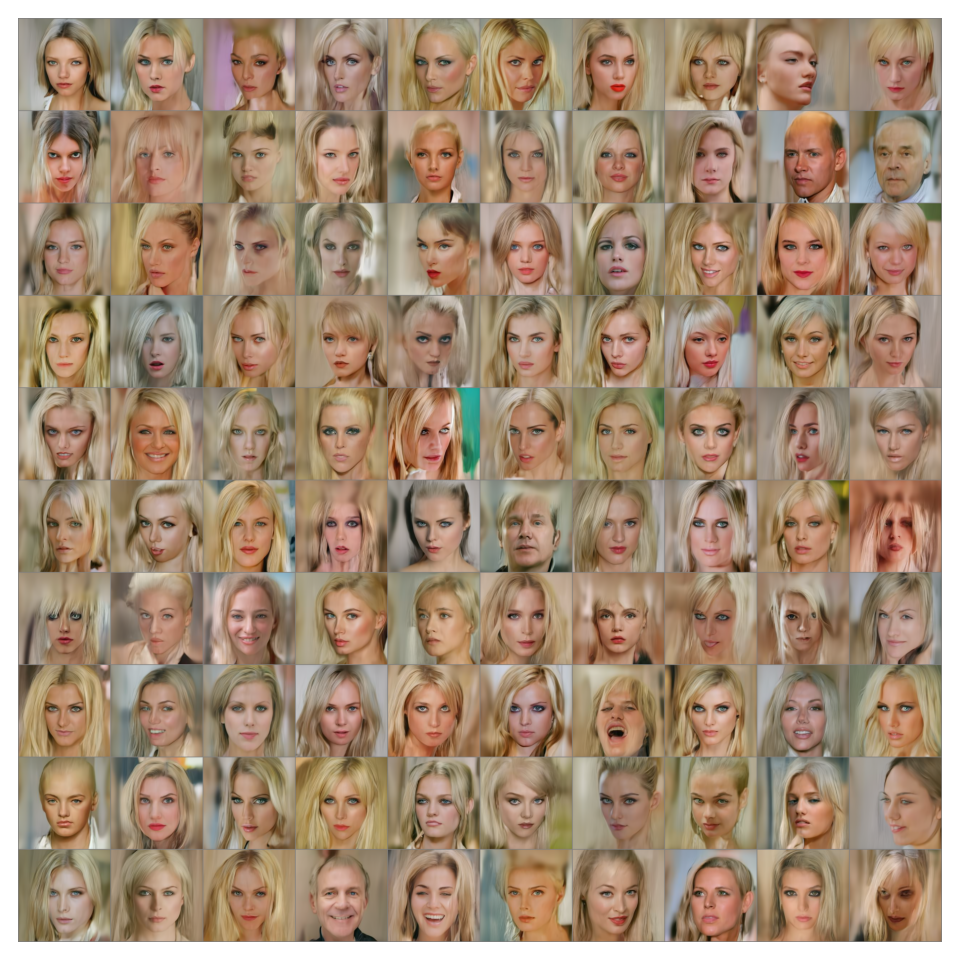
\includegraphics[scale=0.75]{img/results/ddpo-aesthetic-samples.png}
            \vspace{-4pt}  % reduce space between caption and figure
            \captionsetup{width=\textwidth} % set the width of the caption
            \caption{Celeba-HQ 256x256 generated samples from the DDPO finetuned model optimized by aesthetic quality.}
            \label{fig:ddpo-aesthetic-samples}
        \end{figure}

    \newpage

    \section{Implementation details}

    Lalal

    \subsection{Hyperparameters}

    XYZ

	% Tablas
	\enabletablerowcolor[2] % Activa el color de celda
	\begin{table}[H]
		\begin{threeparttable}
		\centering
		\caption{Tabla de cálculo.}
		\begin{tabular}{cccC{4cm}}
			\hline
			\textbf{Elemento} & $\epsilon_i$ & \textbf{Valor} & \textbf{Descripción} \bigstrut \\
			\hline
			A     & 10    & 3,14$\pi$ & Valor muy interesante\tnote{a} \\
			B     & 20    & 6 & Segundo elemento \\
			C     & 30    & 7 & Tercer elemento\tnote{1} \\
			D     & 150    & 10 & Sin descripción \\
			E     & 0    & 0 & Cero \\
			\hline
			\end{tabular}
		\begin{tablenotes}
			\item[a] Este elemento tiene una descripción debajo de la tabla
			\item[1] Más comentarios
		\end{tablenotes}
		\end{threeparttable}
		\label{tab:anexo-1}
	\end{table}
	\disabletablerowcolor % Desactiva el color de celda



\end{appendixs}